
% In your preamble, after \documentclass:
\documentclass[12pt,oneside,openany]{report}
\usepackage[margin=1in]{geometry}
\usepackage{graphicx}
\usepackage{float}


\usepackage[margin=1in]{geometry}
\usepackage{setspace}
\usepackage{titlesec}
\usepackage{graphicx}
\usepackage{tocloft}
\usepackage{fancyhdr}
\usepackage{longtable}
\usepackage{longtable}
\usepackage{calc}
% Page number placement
\pagestyle{plain}
\fancyhf{}
\cfoot{\thepage}
\setlength{\footskip}{0.5in}
\usepackage{amsmath}
% Page numbering
\pagenumbering{roman}
\usepackage{listings}
\usepackage{adjustbox}
\usepackage{float}
\usepackage{enumitem}
\usepackage{minted}

% Set single spacing for Table of Contents
\setcounter{secnumdepth}{2}
\setcounter{tocdepth}{1}

% Title format
\titleformat{\chapter}[block]
{\normalfont\large\bfseries\centering}{\thechapter.}{1em}{\MakeUppercase}


\makeatletter
\let\cleardoublepage\clearpage
\makeatother
\begin{document}
\pagenumbering{roman}     % Start roman numbering
\thispagestyle{empty}     % Suppress page number on title page
% (title page content here)

\clearpage
\begin{singlespace}
\begin{center}
     \hskip 1pt \\
     \hskip 1pt \\    % Title on line 3 - 15 words or fewer, ALL CAPS
     ENHANCING COST EFFICIENCY AND PERFORMANCE OF GPT-4O CHATBOTS: A CASE STUDY ON ACADEMIC ADVISOR SYSTEMS\\
     \hskip 1pt \\
     \hskip 1pt \\
     \hskip 1pt \\
     \hskip 1pt \\    % Name on line 8
     Bulut Tok\\
     \hskip 1pt \\
     \hskip 1pt \\
     \hskip 1pt \\    % Begin statement on line 13
    A Thesis Submitted to the\\
    University of North Carolina Wilmington in Partial Fulfillment\\
    of the Requirements for the Degree of\\
    Master of Degree\\
    \hskip 1pt \\
    \hskip 1pt \\    % Department on line 19
    Department of Computer Science and Information System\\
    \hskip 1pt \\    % UNCW on line 21
    University of North Carolina Wilmington\\
    \hskip 1pt \\    % Year on line 23
    2025\\
    \hskip 1pt \\
    \hskip 1pt \\    % Approved by on line 26
    Approved by\\
    \hskip 1pt \\
    \hskip 1pt \\    % Advisory Committee on line 29
    Advisory Committee\\
    \hskip 1pt \\
    \hskip 1pt \\    % Begin Signature Lines on line 32
\end{center}

% --- Advisory Committee Signature Lines ---
\begin{center}
    Dr. Jeff W. Cummings \hspace{2in} Dr. Laavanya Rachakonda
\end{center}
\vspace{-0.23in}
\rule{2.5in}{.01in} \hspace{1.65in} \rule{2.5in}{.01in}\\




\begin{center}
    % --- Chair signature ---
    Dr. Gulustan Dogan\\[-0.5em]   % moves the rule up closer
    \rule{2.5in}{0.01in}\\[0.5em]
    Chair

    \vspace{2em}  % Some vertical space between the two signature sections

    % --- Accepted by on line 39 ---
    Accepted by\\[0.5em]
    % --- Dean's Signature on line 41 ---
    \rule{2.5in}{0.01in}\\[0.5em]
    Dean, Graduate School
\end{center}
\end{singlespace}

% Front matter
\newpage
\doublespacing
\chapter*{ABSTRACT}
\addcontentsline{toc}{chapter}{ABSTRACT}
\vspace{2ex}

Effective academic advising and personalized course selection are critical yet resource-intensive aspects of higher education. To address this challenge, this thesis presents a comparative analysis of two implementations of an academic advising chatbot built on OpenAI’s GPT-4: a general-purpose base model and a domain-specific fine-tuned model. The fine-tuned model was optimized with targeted academic data derived specifically from the Master of Science in Computer and Information Science (MSCSIS) program, enabling tailored and context-sensitive advising. In contrast, the base model operated without additional domain-specific training.

A systematic evaluation was conducted by posing identical advising queries—covering topics such as curriculum requirements, degree audits, credit completion, and prerequisite verification—to both chatbot configurations. Quantitative metrics, including token consumption, computational complexity, and operational costs, were meticulously recorded and analyzed. The results demonstrated that the fine-tuned model significantly reduced token usage and operational expenses without compromising the accuracy, relevance, or clarity of its responses.

Preliminary assessments utilizing anonymized student academic records confirmed that both models effectively extracted and interpreted critical academic information from structured sources. However, the fine-tuned model consistently showed greater precision and improved contextual alignment specific to the MSCSIS curriculum.

These findings underscore the advantages of domain-specific fine-tuning, illustrating how strategic model customization enhances efficiency, reduces operational costs, and maintains high-quality, personalized interactions. This research provides valuable insights supporting the broader adoption and effective deployment of AI-driven academic advising systems in higher education.

\newpage

\tableofcontents
\clearpage

% 2) List of Tables (separate page)

\addtocontents{lot}{\protect\noindent\textbf{Table}\hfill\textbf{Page}\par\medskip}
\listoftables
\clearpage


% 3) List of Figures (separate page)
\addtocontents{lof}{\protect\noindent\textbf{Figure}\hfill\textbf{Page}\par\medskip}
\listoffigures
\clearpage

% Switch to Arabic page numbering for the main body




\chapter*{NOMENCLATURE}
\addcontentsline{toc}{chapter}{NOMENCLATURE}

\begin{description}[leftmargin=!,labelwidth=\widthof{\bfseries IB Fine Tuning}]

  \item[GPT]
  Generative Pre-trained Transformer, a family of large language models trained on vast corpora of text

  \item[Token]
  The smallest unit of text processed by large language models, where token counts directly affect computational cost

  \item[UUID]
  Universally Unique Identifier, used for session tracking and context management

  \item[LoRA]
  Low-Rank Adaptation, a parameter-efficient fine-tuning technique that reduces the number of trainable parameters

  \item[IB Fine Tuning]
  A strategy focused on retaining critical, task-relevant information while discarding extraneous data

  \item[Meta Prompt]
  A guiding prompt that instructs the model on its role, style, and constraints for generating responses

\end{description}

\clearpage


\pagestyle{fancy}   % Now use the fancy page style for the rest of the document
\fancyhf{}          % Clear any existing header/footer settings
\cfoot{\thepage}    % Set the footer to display the page number

\pagenumbering{arabic}

\chapter{INTRODUCTION}


Deploying advanced chatbot technologies for academic advising requires a careful balance between performance optimization and cost efficiency, especially within specialized graduate programs. This challenge is particularly significant for the Master of Science in Computer and Information Science (MSCSIS) program at the University of North Carolina Wilmington (UNCW), where students frequently encounter complex academic planning decisions due to a diverse range of courses, prerequisites, and concentration areas. Traditional advising methods, though critical, often face constraints related to limited advisor availability, potentially delaying timely academic guidance. To address these limitations, artificial intelligence (AI)-driven chatbots, powered by sophisticated generative language models such as OpenAI’s GPT-40, offer promising solutions that can deliver scalable, immediate, and highly personalized academic support.

This thesis rigorously compares two distinct chatbot configurations based on OpenAI’s GPT-40 model: a \textbf{general-purpose base model}, which relies exclusively on its pre-existing foundational knowledge, and a \textbf{domain-specific fine-tuned model}, extensively trained on tailored academic advising data explicitly curated by MSCSIS program faculty. The fine-tuned model leverages targeted datasets capturing realistic advising scenarios, intricate academic policy details, and representative student-advisor dialogues, enabling it to precisely respond to the nuanced, context-specific queries typical of MSCSIS advising interactions. Conversely, the base model serves as an essential baseline, providing a direct comparison to assess the effectiveness and benefits derived from domain-specific customization and training \cite{openai2024}.

A primary concern when deploying advanced large language models, such as GPT-40, is the significant operational cost associated with their resource-intensive computational demands. To mitigate these costs, this research strategically integrates two key methodologies: \textbf{token optimization} and \textbf{domain-specific fine-tuning}. Token optimization targets computational efficiency by refining input and output prompts to minimize the token count required per interaction without diminishing the accuracy, relevance, or clarity of responses. Given that even incremental reductions in token usage yield substantial cost savings when scaled to numerous student interactions, effective token optimization represents a critical component of the chatbot’s economic sustainability.

Complementing token optimization, domain-specific fine-tuning significantly improves response accuracy and computational efficiency by customizing the GPT-40 model with specialized academic advising datasets. These datasets include realistic dialogues between students and academic advisors, detailed academic policy explanations, nuanced prerequisite clarifications, and complex edge cases specifically relevant to the MSCSIS program. This targeted training greatly enhances the fine-tuned model’s proficiency in interpreting and responding accurately to the distinct terminologies, academic structures, and advising complexities inherent within the MSCSIS academic context. In contrast, the general-purpose base model, devoid of such tailored training, provides a benchmark for evaluating the clear advantages conferred by domain-specific fine-tuning \cite{openai_finetuning_guide}.

To ensure that both chatbot configurations provide context-sensitive and accurate guidance, this project integrates structured academic data sources, including anonymized student records from DegreeWorks, containing critical details such as student identifiers, department affiliations, advisor assignments, GPAs, and academic progress metrics. Additionally, course-specific information—such as course codes, titles, credit hours, scheduling, and detailed prerequisites—is systematically structured in JSON files, enabling both chatbot versions to accurately cross-reference academic records with program requirements. The fine-tuned model particularly excels at extracting, interpreting, and utilizing these structured datasets, consistently generating more precise, personalized, and concise responses tailored to each student’s unique academic situation.

Initial qualitative and quantitative evaluations of both chatbot configurations, conducted using anonymized academic records and structured advising queries, confirm their overall capability to effectively interpret and process essential academic information. Preliminary qualitative tests involved simulated student-advisor dialogues addressing various degree audit scenarios, core course prioritization, and graduation requirements. These assessments revealed that, although both models produced relevant academic recommendations, the fine-tuned model consistently provided responses with enhanced contextual relevance, superior accuracy, and more concise phrasing. Additionally, rigorous quantitative analyses, involving repeated testing across multiple advising scenarios, demonstrated the fine-tuned model’s significant reduction in token usage (approximately 31.5\% fewer tokens compared to the base model) and corresponding operational cost savings, confirming the practical value of strategic domain-specific fine-tuning.

Beyond these computational and economic advantages, the chatbot system is designed explicitly to emulate human-like interactions, offering students real-time, context-aware guidance on essential advising tasks such as course selection, prerequisite verification, credit completion, and comprehensive academic planning. Advanced natural language processing (NLP) tools, including emotion and sentiment analysis techniques, further enhance the advising experience by enabling empathetic, nuanced communication tailored to student emotional states. Consequently, the fine-tuned model effectively integrates informational accuracy with empathetic, supportive advising interactions, significantly enriching the overall user experience.

Despite its current prototype status and limited deployment, the comprehensive comparative analysis presented in this research underscores the potential for broader integration within existing academic advising frameworks. By explicitly comparing the fine-tuned model against the base GPT-40 model, this study demonstrates substantial improvements in advisory accuracy, contextual alignment, computational efficiency, and economic viability achieved through targeted customization and training.

Ultimately, this thesis provides valuable insights into deploying customized, scalable, and economically sustainable AI-driven advising solutions within higher education contexts. The explicit focus on comparing fine-tuned and base model performances not only highlights clear technological advantages but also provides practical guidance for institutions aiming to adopt innovative, data-driven academic support systems. By systematically exploring token optimization, domain-specific fine-tuning strategies, structured data integration, and real-time conversational dynamics, this research advances the broader goal of enhancing academic advising quality, accessibility, and efficiency for graduate students, laying essential groundwork for future advancements in AI-powered educational technologies.


\chapter{RESEARCH QUESTION}

\begin{enumerate}
 \item How do the operational costs of a fine-tuned large language model compare to those of a general large language model for academic advising in the MSCSIS program at UNCW?
\end{enumerate}



\chapter{SCOPE}
The scope of this project is to enhance the academic advising experience for Master of Science in Computer and Information Science (MSCSIS) students at the University of North Carolina Wilmington (UNCW), with a particular emphasis on cost optimization in deploying advanced AI models. The project is designed as a supportive chatbot system that complements traditional advising by providing personalized, efficient, and accessible guidance for complex academic decisions such as course selection, prerequisite verification, and academic progress management. Leveraging advanced natural language processing (NLP) and powered by OpenAI's GPT-40 model, the system delivers real-time responses that integrate seamlessly with UNCW's existing course structures and academic policies.

A key element of the project is the strategic focus on reducing operational costs through methods like token optimization and fine-tuning the model for domain-specific tasks. By refining the input and output prompts to minimize computational overhead and by customizing the model with targeted academic data, the research aims to lower expenses while maintaining high performance and predictive accuracy. Concentrating exclusively on the MSCSIS program, the initiative relies on accurate datasets of course information and student records, with the understanding that the recommendations are based on current data that may evolve over time.

By centering on both the enhancement of academic advising services and the cost-efficient deployment of advanced AI technology, the comparative approach—evaluating the fine-tuned model versus the base model—seeks to deliver a sustainable and scalable solution that optimally supports the academic success of MSCSIS students.

\chapter{REVIEW OF LITERATURE REVIEW AND ANALYSIS}

This section reviews key research on generative AI, with particular emphasis on fine-tuned models of ChatGPT in higher education, and explores their impact on academic advising. Additionally, relevant literature highlighting different approaches on token consumption is examined, alongside related chatbot studies, to provide context and support for this project.

As shown in Table~\ref{tab:comparative-studies}, the comparative studies provide a broad overview of various approaches and applications

\begin{longtable}{|p{2.5cm}|p{4.5cm}|p{4cm}|p{4cm}|}
\caption{Comparative Studies and Applications} \label{tab:comparative-studies} \\
\hline
\textbf{Author(s)} & \textbf{Title of Article} & \textbf{Definition} & \textbf{Relevance to My Work (Advisor Chatbot)} \\ \hline
\endfirsthead
\hline
\textbf{Author(s)} & \textbf{Title of Article} & \textbf{Definition} & \textbf{Relevance to My Work (Advisor Chatbot)} \\ \hline
\endhead
\endhead

 Laura Villa et all. &Comparative Analysis of Generic and Fine-Tuned Large Language Models for Conversational Agent Systems & The paper highlights trade-offs between immediate applicability (G-GPT) and long-term precision (FT-GPT), insights vital for applications like customer support, healthcare, or education that require accuracy, dynamic entity handling, and precise intent recognition. It also notes inherent GPT biases, stressing the need for careful dataset curation and review processes. \cite{robotics13050068} & TThis study indicates that improved accuracy in intent classification and entity extraction is achieved through the use of fine-tuned GPT models, and that precision and contextual relevance are enhanced by the incorporation of domain-specific datasets. The effective management of dynamic entities is also demonstrated, with these outcomes serving to validate the methodological approach employed in the fine tuned system.
\\ \hline
Ting Fang Tan &Fine-tuning Large Language Model (LLM) Artificial Intelligence Chatbots in Ophthalmology and LLM-based evaluation using GPT-4 & This article reports on a study where researchers fine-tuned several large language models (LLMs) to answer ophthalmology-related patient queries and then evaluated their performance using both an automated GPT-4–based evaluation framework and human clinician rankings.\cite{tan2024fine} & The study highlights the benefits of fine-tuning LLMs for domain-specific applications. It demonstrates that fine-tuning enhances the model’s accuracy and relevance in responding to specialized queries. 
\\ \hline
Tingxu Han&Token-Budget-Aware LLM Reasoning & This article addresses the challenge of high token usage—and thus increased cost and latency—in Chain-of-Thought (CoT) reasoning with large language models (LLMs). Although CoT prompts help models reason through problems by breaking them into intermediate steps, they often produce unnecessarily lengthy outputs.\cite{han2024token} & Both works focus on reducing token consumption to lower computational costs while maintaining performance. TALE achieves this by dynamically controlling the token budget during reasoning, whereas the system demonstrates that fine-tuning can significantly cut token usage in a practical academic advising chatbot.
\\ \hline
\\ \hline
Shivanshu Shekhar& Towards Optimizing the Costs of LLM Usage & TThis article introduces QC-Opt, a framework that reduces LLM usage costs by predicting output quality without invoking the models, then optimally routing queries to the most cost-effective LLMs, and finally applying quality-aware token reduction techniques. The approach balances cost, latency, and quality—achieving significant cost savings  and modest improvements in output quality for tasks such as document summarization.\cite{shekhar2024towards} & This article focusing on quality-aware token optimization and cost-efficient model routing is highly relevant to the system, which also aims to reduce token usage and operational expenses..
\\ \hline
Ganesh Reddy Gunnam &The Performance and AI Optimization Issues for task oriented chatbots & This study emphasizes that integrating robust NLU services and refining keyword detection algorithms enhances both response accuracy and overall system efficiency. He advocates for a hybrid machine learning approach—combining models like BERT with intent prediction frameworks—to boost the performance of task-oriented chatbots.\cite{gunnam2024performance} & The study details various testing methodologies and performance metrics that help assess communication efficiency and system reliability.
\\ \hline
Abdulrahman Alkhoori et al. (2024) & UniBud: A Virtual Academic Adviser & Discusses the design and implementation of UniBud, a virtual academic advisor using natural language understanding for answering common student queries. Focuses on usability and task efficiency.\cite{9099191} & Provides insights on improving usability and efficiency, which are key considerations for developing an advisor chatbot. \\ \hline
P. S. Aithal \& S. Aithal (2023) & Application of ChatGPT in Higher Education and Research – A Futuristic Analysis & Examines the applications of ChatGPT in higher education, focusing on its impact, challenges, and opportunities in academic and research settings.\cite{chatgpt_higher_education_ssrn} & Highlights potential use cases and challenges of integrating AI tools in education, directly relevant for enhancing an advisor chatbot’s role. \\ \hline
Yun Dai et al. (2023) & ChatGPT: A Student-Driven Innovation in Education & Conceptualizes ChatGPT as a student-centric innovation that enhances personalized learning, real-time feedback, and accessibility in education.\cite{dai2023} & Provides a framework for integrating ChatGPT into academic systems to offer personalized and accessible advising services. \\ \hline
Thottoli, Mohammed et al. & Robo-Academic Advisor: Can Chatbots Replace Human Interaction? & Explores the potential and limitations of chatbots and AI in academic advising, focusing on scalability and ethical concerns.\cite{thottoli2024robo} & Addresses the importance of balancing automation with ethical considerations in developing advisor chatbots. \\ \hline
Kasra Lekan, Zachary A. Pardos (2023) & AI-Augmented Advising: A Comparative Study of GPT-4 and Advisor Recommendations & Analyzes the use of GPT-4 for major recommendations in academic advising, comparing its effectiveness with human advisors.\cite{lekan2024aiaugmented} & Provides evidence of how GPT-4 can augment academic advising, supporting the development of AI-driven advising systems. \\ \hline
Ronit Banerjee, Kathryn Butziger, Jose Fabrizio Filizzola Ortiz, and
Matthew Kiszla. (2023) & Customizing Large Language Models for Automated Academic Advising at Universities & Investigates the customization of large language models like GPT-4 for academic advising through fine-tuning and prompt engineering.\cite{banerjee_2024} & Offers technical insights on tailoring GPT models to meet the specific needs of an advisor chatbot. \\ \hline

\end{longtable}


\section{ChatGPT and Generative AI in Higher Education}

Generative AI has increasingly shown potential in education, particularly through personalized support for academic tasks. Akiba and Fraboni explore how AI tools like ChatGPT can make academic advising more accessible and efficient by providing high-quality, comprehensive responses \cite{educsci13090885}. This work highlights the complementary role of AI alongside human advisors, particularly in improving access to timely, personalized guidance\cite{educsci13090885}. the system created applies this model by offering real-time academic support tailored to the individual needs of MSCSIS students, providing a more accessible advising experience.

The use of AI in education, while promising, also presents challenges such as the potential devaluation of skills and the risk of inaccuracies. Steele  addresses these concerns by discussing how AI can empower students by supporting critical thinking and problem-solving skills through knowledge aggregation and genre understanding \cite{STEELE2023100160}. AI systems like the system created similarly aim to assist students in navigating complex academic decisions, complementing traditional advising approaches and enhancing student autonomy in academic planning.

Custom GPT models have proven effective in strategic decision-making in higher education, offering institutions valuable insights for academic and administrative planning \cite{chukhlomin2024}. Chukhlomin emphasizes that while AI can generate useful recommendations, human expertise is essential for interpreting these outputs and aligning them with institutional objectives \cite{chukhlomin2024}. This principle resonates with the the system created system, which combines AI-driven insights with the expertise of human advisors to provide personalized academic recommendations for students.


\section{Fine-Tuning for Cost Efficiency, Accuracy and  Performance Enhancement}

Fine-tuning large language models (LLMs) like GPT-4o is crucial for enhancing both cost efficiency and overall performance in specific applications such as academic advising. By tailoring the model to the unique requirements of the fine tuned system, fine-tuning not only enables the generation of more accurate and relevant responses but also reduces the computational resources needed.

Zhang et al. demonstrated that fine-tuning LLMs on targeted datasets significantly improves performance in specialized tasks, reducing the need for extensive prompt engineering and lowering token usage \cite{D4SC00924J}. This approach is especially effective in cutting operational costs, as the model becomes more efficient at producing precise responses with fewer tokens \cite{D4SC00924J}. Research in chemical data extraction further demonstrates that fine-tuning large language models can effectively bridge the gap between natural language understanding and the rigorous demands of extracting structured data in chemical research \cite{D4SC00924J}. By achieving high accuracy with relatively modest annotated datasets and reducing reliance on extensive prompt engineering, this method lays a robust foundation for more automated, efficient, and scalable text mining, underscoring the broader potential of fine-tuning techniques to optimize systems where precise data extraction underpins effective decision-making.

Studies have also shown that prompt engineering can serve as an effective alternative to fine-tuning for achieving high performance in domain-specific tasks. For instance, Zhang et al. conducted a comparative analysis of prompt engineering and fine-tuning strategies in large language models for classifying clinical notes—specifically, identifying patients with metastatic cancer from discharge summaries \cite{Zhang2024Comparison}. Their findings revealed that clear, concise prompts incorporating reasoning steps significantly boosted performance, with GPT-4 exhibiting superior accuracy among all models tested \cite{Zhang2024Comparison}.

Fine-tuning also minimizes reliance on generic language patterns, allowing the fine tuned system to concentrate on the specific language and structures pertinent to academic advising. This targeted optimization improves the quality of the advice provided while streamlining the computational process, resulting in faster response times and reduced costs. Integrating domain-specific knowledge further enhances predictive accuracy. For the fine tuned system, the incorporation of MSCSIS-specific academic data ensures that students receive accurate, personalized advice—including tailored course recommendations and precise prerequisite checks. Liu et al. emphasize that domain-specific knowledge is essential for adapting LLMs for educational applications, thereby improving their ability to deliver relevant and accurate responses \cite{Liu_2023}.

Fine-tuning LLMs with domain-specific datasets through parameter-efficient techniques such as LoRA and QLoRA has been shown to improve performance in specialized applications while reducing output token usage \cite{jeong2024fine}. When applied to academic advising for MSCSIS students, models that capture the distinctive language and contextual nuances of the field yield more concise, context-aware responses. This reduction in output tokens minimizes computational overhead and lowers operational costs without compromising response quality, highlighting the potential for an academic advisor chatbot that is both economically efficient and tailored to its users' unique needs.

The use of fine-tuning techniques for adapting LLMs to specialized domains has garnered considerable attention in recent research. Anisuzzaman et al. present a comprehensive review of fine-tuning approaches—including supervised methods, reinforcement learning from human feedback, and parameter-efficient strategies such as QLoRA \cite{anisuzzaman2024fine}. Although their review primarily focuses on applications within the medical field, the methodologies and challenges discussed—such as managing domain-specific data, mitigating hallucinations, and optimizing computational resources—are directly applicable to academic advising. These insights reinforce the potential for enhancing model performance while controlling operational costs, a central goal in developing the fine tuned system.

Pareja et al. (2025) provide a comprehensive study on the supervised fine-tuning of small language models, emphasizing cost efficiency and accessibility for resource-constrained developers \cite{pareja2024unveilingsecretrecipeguide}. Their systematic exploration of various hyperparameter configurations, such as batch size, learning rate, and training strategies, demonstrates that larger batch sizes paired with lower learning rates can significantly enhance model generalization and sample efficiency. Their findings suggest that simpler, stacked training approaches can yield competitive performance while reducing computational overhead, directly supporting the development of the fine tuned system through similar fine-tuning strategies and hyperparameter optimizations.

Touvron et al. introduce Llama 2, an open foundation of pretrained and fine-tuned large language models optimized for dialogue applications \cite{touvron2023llama2openfoundation}. Their work demonstrates that careful fine-tuning, as applied in the Llama 2-Chat models, can substantially enhance conversational performance, safety, and reliability while maintaining cost efficiency. This approach aligns with the methodology used in the fine tuned system, where fine-tuning techniques—similar to those implemented in GPT-4o—are leveraged to increase the accuracy, reliability, and cost-effectiveness of the academic advising chatbot. Adapting a general-purpose language model through supervised fine-tuning highlights the value of tailoring model outputs to meet domain-specific needs, enabling robust and scalable AI-driven solutions.

Finally, Taherkhani et al. highlighted that fine-tuning reduces the necessity for complex prompt designs, which are often resource-intensive \cite{taherkhani2024epiccosteffectivesearchbasedprompt}. By leveraging fine-tuning, the fine tuned system can achieve high levels of accuracy and efficiency without incurring the additional costs associated with prompt engineering.


\section{Optimizing Tokens for Cost Efficiency}

Token optimization plays a critical role in enhancing the cost efficiency of large language models. By streamlining token usage, the fine-tuned system created not only reduces the computational load but also lowers operational expenses, thereby making the system more sustainable and scalable. Han et al. explored how optimizing token distribution can improve processing efficiency by reducing the reliance on long-tail tokens that contribute minimally to model performance \cite{han2023understandingincontextlearningsupportive}. In the context of the system created, this strategy ensures that the model generates concise and relevant responses without unnecessary verbosity.

Recent studies further underscore the benefits of token optimization. Zhang et al. found that GPT-4 maintained high accuracy even when key terms were removed or parts of the input were randomly discarded, highlighting the model's robustness to incomplete data. This observation suggests that dynamic token optimization—implemented via real-time prompt adjustment—can effectively minimize token usage without compromising predictive performance \cite{Zhang2024Comparison}. Complementing this approach, Lin et al. propose a method for LLM-based recommendation that leverages influence and effort scores to select representative samples for few-shot fine-tuning. Their method prunes the training dataset to reduce computational overhead while maintaining high performance \cite{lin2024data}. This approach aligns closely with the fine-tuning configurations in system, where selecting high-value data samples is crucial to balancing precision and cost efficiency.

In resource-constrained environments, innovative fine-tuning strategies such as IB fine-tuning have proven effective in retaining critical task-relevant information while eliminating redundant data, thereby reducing computational costs without sacrificing accuracy \cite{jo2025efficiency}. Further supporting the economic viability of these techniques, Bergemann, Bonatti, and Smolin present an economic framework that analyzes token allocation, fine-tuning, and optimal pricing for LLM services. Their model, which considers the variable costs of processing input, output, and fine-tuning tokens, links technical improvements directly to market pricing \cite{bergemann2025economics}.

Finally, advancements in tokenization further enhance overall system performance. GPT-4o's advanced tokenizer, as discussed by Islam and Moushi, facilitates faster and more efficient tokenization processes \cite{Islam_2024}. This efficiency reduces the number of tokens required to convey meaningful information, thereby lowering the cost per interaction. By integrating these token optimization techniques, the fine-tuned system can handle more queries with the same computational resources, ultimately improving both cost efficiency and response times for students seeking academic advice.



\section{Additional Contributions to Generative AI in Education} 

Interdisciplinary research is crucial in ensuring the responsible integration of AI in education \cite{arxiv230518086}. Gabashvili  advocates for continuous evaluation of AI tools to address emerging ethical and practical challenges \cite{arxiv230518086}. This is particularly relevant to AI-driven advising systems like academic advising chatbot system, which must remain adaptable to ensure they meet ethical standards and provide reliable academic support.

Conversational AI has proven transformative in simplifying decision-making processes, particularly in educational settings \cite{bdcc7020062}. Hassani and Silva  examine how AI tools like ChatGPT can streamline complex decisions by offering real-time, relevant information \cite{bdcc7020062}. This ability to simplify decision-making aligns with the advising system's goal of providing MSCSIS students with timely, personalized advice that enhances their academic planning.

Ethical concerns are central to the deployment of AI in education, particularly in ensuring fairness and transparency \cite{su15075614}. Kooli  highlights the need for ethical standards to guide the use of AI chatbots in educational contexts \cite{su15075614}. These principles are integral to systems like advising system created, which emphasizes transparency in its interactions and prioritizes the protection of student data and privacy.

AI systems are increasingly being used to facilitate student help-seeking behaviors by lowering barriers to accessing support \cite{Merikko2024AnAA}. Merikko and Silvola explore how AI agents can encourage students to seek assistance, a role that reflects broader efforts in educational AI systems \cite{Merikko2024AnAA}. The system created adopts a similar approach by providing students with easy access to academic advice, ensuring that support is available when needed.

The potential for AI-generated responses to provide empathetic support is becoming more apparent, particularly in educational settings \cite{inaba2024largelanguagemodelsused}. Inaba  demonstrate how AI responses can match human counselors in providing empathetic feedback, especially in role-play scenarios \cite{inaba2024largelanguagemodelsused}. These insights benefit academic advising systems like adviisng system's, which improve student engagement with both informative and supportive interactions.

\chapter{DATA SET}

The development of the system  relies on several key datasets that form the core of its academic advising capabilities. These data sources—including a comprehensive course information repository and detailed insights into student academic progress—are processed and integrated into the chatbot’s architecture. Additionally, a  fine-tuning dataset, capturing a wide range of realistic advising scenarios, further enhances its ability to provide accurate, real-time academic advice to MSCSIS students at the University of North Carolina Wilmington (UNCW).

\section{Primary Datasets}

\subsubsection{JSON Cache File: Course Data}
This dataset is derived directly from the university’s official course catalog and is organized in a clear, structured format. It provides detailed course information including course codes, titles, full descriptions, and scheduling details such as meeting times, locations, and session types. In addition, it includes important attributes like credit hours, prerequisites, restrictions, and course repeatability, ensuring that all essential information for academic advising is readily available.

\subsubsection{PDF Documents: Degree Audits}
The degree audit documents offer a detailed snapshot of a student’s academic progress by outlining both completed and pending degree requirements. They provide clear insights into a student’s current standing and include supplementary context—such as course recommendations, academic policies, and additional notes—that enriches the advising process and enables more personalized guidance.

\section{Fine-Tuning Data}
To enhance system performance and token efficiency, the fine-tuning dataset employs concise conversation examples specifically designed to provide clear, brief responses to diverse advising scenarios. It encompasses:

\begin{itemize}
\item \textbf{Edge Cases and Policy Information:} Examples address complex scheduling conflicts, credit load challenges (e.g., situations where students seek fewer credits than required), and detailed policy-related questions, enabling the chatbot to adeptly navigate nuanced advising issues.
\item \textbf{Short Answers for Token Reduction:} The dataset prioritizes short, precise answers to minimize token usage. This strategy ensures the chatbot remains both effective and economical, rapidly addressing inquiries without compromising clarity.
\item \textbf{Routine and Complex Scenarios:} The fine-tuning includes examples of both standard interactions and challenging questions, totaling numerous scenarios that help maintain robust performance across various contexts.
\end{itemize}


Examples from training file:

\section{Fine-Tuning Examples}

\begin{itemize}

\item \textbf{Scenario 1: Credit Hours Requirement}
\begin{lstlisting}[breaklines=true]
{"messages": [
    {"role": "system", "content": "academic advisor"},
    {"role": "user", "content": "What happens if I take less than 9 credit hours in a semester?"},
    {"role": "user", "content": "retrieved_data: CACHE_FILE: course_index_cache.json"},
    {"role": "user", "content": "Relevant PDF: Advising information stresses that full-time status requires at least 9 credit hours."},
    {"role": "user", "content": "JSON Excerpts: {\"full_time\": {\"min\": 9}}"},
    {"role": "assistant", "content": "If you take fewer than 9 credits, you'll lose your full-time status, affecting academic progress and possibly visa status."}
]}
\end{lstlisting}

\item \textbf{Scenario 2: Graduation Credit Status}
\begin{lstlisting}[breaklines=true]
{"messages": [
    {"role": "system", "content": "You are an academic advisor."},
    {"role": "user", "content": "What is my credit status if I have 35 credits earned?"},
    {"role": "user", "content": "retrieved_data: CACHE_FILE: course_index_cache.json"},
    {"role": "user", "content": "Relevant PDF: Degree audit indicates \"Credits applied: 35 | Credits required: 36\""},
    {"role": "user", "content": "Course Info: Total required credits: 36."},
    {"role": "assistant", "content": "You've earned 35 credits and are just 1 credit short of graduation."}
]}
\end{lstlisting}

\item \textbf{Scenario 3: Course Description}
\begin{lstlisting}[breaklines=true]
{"messages": [
    {"role": "system", "content": "academic advisor"},
    {"role": "user", "content": "Summarize BAN510 - Sports Analytics for me."},
    {"role": "user", "content": "retrieved_data: CACHE_FILE: course_index_cache.json"},
    {"role": "user", "content": "Relevant PDF: BAN510 is described as an introductory course in sports analytics using modern analytics techniques and tools."},
    {"role": "user", "content": "JSON Excerpts: {\"course\": \"BAN510 - Sports Analytics\", \"detail_url\": \"https://catalogue.uncw.edu/preview_course.php?catoid=74&coid=277765\", \"description\": \"Introduces fundamental analytics concepts in sports, with emphasis on using analytics tools to add competitive advantage.\", \"Credit Hours\": \"3\"}"},
    {"role": "user", "content": "Course Info: No schedule information available."},
    {"role": "assistant", "content": "BAN510 - Sports Analytics is a 3-credit introductory course covering key analytics concepts and tools to enhance competitiveness in sports."}
]}
\end{lstlisting}

\item \textbf{Scenario 4: Thesis Submission Documentation}
\begin{lstlisting}[breaklines=true]
{"messages": [
    {"role": "system", "content": "academic advisor"},
    {"role": "user", "content": "Before I submit my final thesis, what documentation do I need?"},
    {"role": "user", "content": "retrieved_data: CACHE_FILE: course_index_cache.json"},
    {"role": "user", "content": "Relevant PDF: Required documents include Draft Thesis, Format Approval Sheet, Final Thesis, Signed Thesis Title Page, ETD Submission Form."},
    {"role": "user", "content": "Course Info: These documents are mandatory for thesis submission."},
    {"role": "assistant", "content": "You'll need your Draft Thesis with a Format Approval Sheet, Final Thesis, Signed Title Page, and ETD Submission Form. Ensure you also apply for graduation."}
]}
\end{lstlisting}

\end{itemize}







Together, these datasets empower our academic advising tool to deliver personalized, accurate, and context-sensitive guidance that meets the diverse needs of our student population. This data-driven approach ensures students receive accurate advice based on the latest course offerings and academic requirements.


% Methodology
\chapter{METHODOLOGY}
This section outlines the design, development, and integration of a conversational academic advising system.This study presents two identical systems for academic advising that differ solely by the model variant employed: one system uses a fine-tuned GPT-based model, while the other uses a non-fine-tuned baseline model. The primary objective is to compare the cost and token consumption between these two configurations under identical operational conditions.

\section{Data Integration and Processing}
The system begins by integrating multiple sources of information to generate context-aware academic advising. Course-related data is primarily obtained from a cache file, which serves as the main knowledge base. Additionally, users have the option to upload PDF files that provide supplementary context. The data sources are as follows:

\begin{itemize}
 \item Cache File: The cache file is our primary data source, containing structured course information essential to generate academic advice.
 
 \item PDF Data: PDF files are processed using the PyPDF2 \cite{PyPDF2} library to extract text, thereby enriching the contextual background with additional details.
\end{itemize}

All text inputs are preprocessed by removing markdown formatting and sanitizing harmful characters, including SQL-sensitive symbols, to ensure safe and reliable analysis. Furthermore, the system conducts sentiment and emotion analysis using NLTK’s VADER \cite{nltkSentiment} and a Hugging Face emotion classifier \cite{huggingface_models_libraries}, allowing it to adjust responses based on the user’s emotional tone.

In the system, course data is obtained from a JSON cache and then embedded directly into the conversation history as part of a system prompt. This ensures that the information used to answer user queries is rendered complete and verifiable, relying solely on the explicit course data provided. Additionally, if any PDF context is available, it is appended as further system information, thereby reinforcing the commitment to using only documented and accurate sources. In contrast to methods that might allow for the inference or generation of supplementary details, any information beyond what is explicitly supplied is deliberately avoided, so that a rigorous standard of academic integrity and precision in data representation is maintained.

\section{Model Selection and NLP Integration}

Two versions of the academic advising system have been implemented, differing solely by the language model employed. One version utilizes a fine-tuned GPT-based model, specifically designed to provide detailed and context-aware academic guidance tailored to MSCSIS students, while the other relies on a baseline, non-fine-tuned GPT model \cite{openai2024}. Both models are accessed via the OpenAI ChatCompletion API using identical generation parameters—including temperature, \verb|top_p|, frequency, and presence penalties \cite{openaiTextGeneration}. By maintaining consistent parameters across both models, any observed variations in response quality, token usage efficiency, or overall cost can be attributed directly to the impact of fine-tuning.

To ensure accurate and personalized advice, the system created integrates diverse data sources into a comprehensive prompt presented to the GPT-4o model. The prompt combines structured academic data—such as course schedules, catalog entries, prerequisites, and detailed information from the course catalog—with student-specific context derived from individual academic records, particularly degree audits provided as PDF files for MSCSIS students. These degree audit files are processed to extract critical information, including completed and pending course requirements, enabling the chatbot to generate highly personalized responses. Additionally, the system handles specific student queries by directing them to appropriate graduate forms or resources, such as forms for continuous enrollment or maintaining full-time student status.

To ensure safety and reliability, the system employs rigorous text sanitization practices. Dedicated functions remove Markdown formatting and sanitize user inputs for SQL safety, effectively preventing injection attacks and ensuring secure interactions. Additionally, the NLP component incorporates sophisticated emotion analysis tools, including the NLTK VADER lexicon and a Hugging Face-based emotion classifier. These tools assess the emotional tone of student queries, identifying negative sentiments such as frustration or anxiety. When significant negative emotions are detected, the system dynamically includes empathetic guidance within the prompt, instructing the GPT model to respond with heightened sensitivity and understanding.

By combining fine-tuned NLP models with structured academic data and context from MSCSIS degree audits, the system created effectively delivers precise, context-sensitive, and empathetic academic guidance. The controlled experimentation between the fine-tuned and baseline GPT models further isolates the impact of fine-tuning, enabling clear insights into performance differences and potential advantages offered by model customization.


\section{Memory Management} 

The chatbot architecture employs robust session management techniques combined with efficient SQL-based data storage to ensure personalized and contextually coherent interactions with users. Sessions within the system are uniquely identified through universally unique identifiers (UUIDs), generated using Python’s built-in uuid library\cite{pythonUUID}. These UUIDs provide a reliable mechanism for distinguishing and maintaining individual user interactions over multiple exchanges. Each conversational turn, including the user's queries and the system’s generated responses, is persistently recorded into a MySQL relational database, facilitated by Python’s mysql.connector library \cite{mysql_connector_python_example_connecting}. The database connection is established securely using defined credentials, ensuring stable and reliable interaction with the underlying MySQL database. To maintain high standards of security and integrity, the system sanitizes user inputs by employing regular expressions designed to remove potentially harmful characters, thereby effectively guarding against SQL injection vulnerabilities \cite{pokhrel2024building}. Each interaction, composed of the sanitized user query and the corresponding chatbot response, is systematically stored into dedicated database tables. This structured approach enables the system to retain conversation history, facilitating continuous dialogue and allowing the chatbot to reference previous conversations effectively, thus providing tailored recommendations and enhanced user engagement over time.


\section{Data-Driven Personalization and Response Generation}

The advising system’s ability to generate personalized responses is rooted in its integration of structured data and NLP. When a student asks about a specific course, the chatbot cross-references the course details with the student’s academic history to check prerequisites and recommend next steps. The system tracks the student’s completed, in-progress, and planned courses, ensuring that the advice aligns with the student’s academic trajectory.

For example, when a student inquires about enrolling in a course, the chatbot checks whether the prerequisites have been met. If any prerequisites are missing, the system provides suggestions for alternative courses or next steps to fulfill those requirements. Additionally, the chatbot tracks the student’s earned and in-progress credits, helping them stay on course to meet graduation requirements.

By combining real-time data processing with the powerful language generation capabilities of GPT-4o, the system created  offers a dynamic and personalized advising experience. The system’s ability to adapt its responses based on the student’s academic history and current standing ensures that each interaction is relevant and valuable.

\section{Prompt}

The system employs a concise meta prompt that directs the language model to serve as an academic advisor for university students. This prompt outlines key responsibilities, including analyzing academic interests, performance, and career goals; offering actionable advice on course selection, research opportunities, internships, and career trajectories; and ensuring responses are structured in clear markdown with headings, bullet points, and summaries. It also provides specific instructions for scenarios such as advising new students, guiding international students on full-time enrollment, addressing capstone queries, and clarifying prerequisite eligibility.Metadata is incorporated to organize and contextualize the information, enabling efficient retrieval and ensuring that the advising responses are both targeted and relevant to each student's unique profile. The use of metadata further increases the accuracy of the output by enhancing the model's ability to reference and align context-specific details, ultimately refining the precision and reliability of the advice provided \cite{ha2023meta}.

 The initial set of Meta prompts is shown below:

 \begin{lstlisting}[ breaklines=true]
# Define the academic advisor meta prompt.
META_PROMPT = """
Act as an academic advisor for university-level students seeking guidance on academic and career planning.

You will help students by analyzing their academic interests, performance, and career goals, and then provide actionable advice on course selection, research opportunities, internships, and career trajectories. Focus on clarity, actionable steps, and evidence-based recommendations. Use reasoning to outline your thought process and then provide your conclusions at the end.

If a new student is asking what they should take, tell them they should start with their core courses.

If an international student wants to be considered full time they should take at least 9 hours and at least 6 in-person credit hours and point them to this website: https://catalogue.uncw.edu/content.php?catoid=74&navoid=10022&hl=%22full+time%22&returnto=search#Full-Time_Status

If they ask "What do I need to register for full time if I am not taking a course but still need to finish my capstone?" point them to this website: https://uncw.edu/myuncw/academics/graduate-school/forms and recommend them to register for continuous enrollment

If they ask "How many capstone hours should I register for?" tell them "3 hours of the capstone is the typical amount to take per semester. The idea is 3 hours during one semester to work on the proposal and 3 hours the following semester to complete/defend the capstone."

If students meets even if only one prerequiste for a course which requires multiple prerequiste, tell them they are eligible.

# Steps

1. Evaluate the student's current academic status and interests.
2. Identify relevant academic and career goals.
3. Provide structured advice on course selection, research opportunities, and career options.
4. Summarize the reasoning process before presenting final recommendations.

# Output Format

The output should be a well-organized response in markdown. Include clear sections with headings, bullet points for actionable steps, and a summary of conclusions at the end. If structured data is required, use JSON format without wrapping it in code blocks.
""".strip()
\end{lstlisting}

The base system prompt builds on this by appending the meta prompt with operational directives and real data. It integrates course information from a JSON cache and any additional PDF context, ensuring that responses are grounded solely in the provided data. The prompt also instructs the model to indicate when specific details (like course schedules or lecturer information) are unavailable, and to direct students to external resources—such as the Graduate School Forms page—when needed.


 The initial set of prompts is shown below:

\begin{lstlisting}[language=Python, breaklines=true]
system_messages = [
    {
        "role": "system",
        "content": (
            META_PROMPT + "\n\n" +
            "You are a helpful and friendly academic assistant with complete and accurate course data. "
            "Below is the course data from a JSON cache. "
            "Answer questions based solely on this provided data and any additional PDF context, "
            "and do not generate or assume any information that is not explicitly provided. "
            "If a course does not include schedule or lecturer information, do not list any lecturers; "
            "instead, state that no lecturer information is available.\n\n"
            f"Course data:\n{json.dumps(courses_dict, indent=2)}\n\n"
            "Additional instructions:\n"
            "For more detailed instructions and to access the necessary forms, visit the [Graduate School Forms](https://uncw.edu/myuncw/academics/graduate-school/forms) page.\n\n"
            "If additional PDF information is provided, take it into account, but do not invent details that are not present."
        )
    }
]
messages = system_messages + user_messages
\end{lstlisting}



\section{Fine-Tuning the Language Model}


The fine-tuning process begins with training and validation files prepared in JSONL format, with 80 percent of the data allocated for training and 20 percent for validation. The training file consists of 177 examples, while the validation file includes 42 examples. This split helps the model learn effectively while providing insights into generalization capabilities. To create these datasets, the JSONL-formatted data is first read and randomized to ensure the absence of bias toward any specific sequence of entries. The data splitting process is executed programmatically in Python using an 80-20 split, where the Python script calculates the exact split index based on dataset size:

\begin{verbatim}

Calculate split index for 80% training and 20% validation

split_index = int(len(examples) * 0.8)
training_examples = examples[:split_index]
validation_examples = examples[split_index:]
\end{verbatim}

These subsets are saved as separate files, designated explicitly as training1.jsonl and validation1.jsonl, and then uploaded via OpenAI's file management system for fine-tuning.

For this purpose, the \texttt{gpt-4o} engine is used. The training dataset includes sample dialogues between students and academic advisors, covering a variety of common queries, edge cases, and UNCW-specific academic policies \cite{openai_finetuning_guide}. Each example in the dataset will follow a structured conversational format, which includes different roles such as \textit{system}, \textit{user}, and \textit{assistant} to provide a clear context \cite{openai_finetuning_guide}.

Following the upload, a fine-tuning job is initiated through OpenAI’s API. This involves specifying particular hyperparameters crucial to the training process. In this implementation, hyperparameters such as a learning rate multiplier of 0.1 and a batch size of 8 are used \cite{openai_finetuning_guide}. These parameters are  selected to balance the trade-off between model convergence and overfitting. The model employs default epoch settings initially, enabling the assessment of baseline model performance before further tuning adjustments.

Monitoring is an essential phase of the fine-tuning process. A Python script continuously polls the job status, capturing important metrics such as training loss, validation loss, and full validation loss, extracted from periodic event logs generated by the OpenAI API \cite{openai_finetuning_guide}. This extraction is performed by parsing descriptive messages that explicitly report these metrics at various stages, helping to evaluate the model’s learning progression:

\begin{minted}[
    frame=single,       % Single-line box around code
    fontsize=\small,    % Adjust font size
    breaklines=true,    % Wrap long lines
    autogobble=true,    % Automatically remove common leading spaces
    xleftmargin=1em     % Extra left margin (optional)
]{python}
def extract_metrics(message):
    metrics = {}
    try:
        if "training loss=" in message:
            part = message.split("training loss=")[1]
            metrics["training_loss"] = float(part.split(",")[0])
            metrics["validation_loss"] = float(part.split("validation loss=")[1].split(",")[0])
            metrics["full_validation_loss"] = float(part.split("full validation loss=")[1].split()[0])
    except Exception:
        pass
    return metrics
\end{minted}


These metrics are critical for diagnosing model performance and identifying the best-performing model iteration, particularly by tracking reductions in full validation loss. The process employs a seed value (seed=42) to ensure reproducibility across runs. The fine-tuning job successfully completed after 67 training steps, achieving a training loss of 1.10, a validation loss of 1.45, and a full validation loss of 1.52.

Upon successful fine-tuning, the performance of the newly fine-tuned model is systematically compared with the base model (GPT-4o) using identical prompts. This direct comparison helps quantify improvements in responsiveness and accuracy, informing decisions on potential future hyperparameter adjustments such as altering epochs, learning rates, or batch sizes based on observed performance metrics. Adjustments to these hyperparameters may be iteratively applied in subsequent tuning cycles to achieve optimal results, guided by empirical observations of loss metrics and generated output quality.


\section{Token Calculation and Cost Optimization}

The token calculation methodology begins by encoding text using the tiktoken library, which converts input text into tokens based on a specified model \cite{tiktoken033}. In the provided implementation, the "gpt-4o" model is used for encoding. If this model is not recognized, the code falls back to using the \verb|cl100k_base| encoding \cite{tiktoken033}. This ensures that token counting remains reliable regardless of the model selected.

For scenarios where multiple text files need to be processed, a folder selection dialog is used to allow the user to choose a directory containing .txt files. Each file is read and processed individually; before tokenization, specific substrings—such as interface prompts ("Ask about courses (or type 'exit' to quit)" and "Assistant: ")—are removed to ensure that only the relevant content is counted.

The Input token cost category pertains to tokens generated by user queries at a rate of \verb|$|2.50 per million tokens \cite{openaiAPIPricing}. User queries yielded token counts ranging from 27 to 56 tokens per question, with the associated total costs computed based on each identical question being asked 10 times for each model. These input costs directly reflect the financial implication of user interactions, in Table~\ref{tab:cost-summary}  (see formula below).

\[
\text{Cost Input} = \left(\frac{\text{input token count}}{1,000,000}\right) \times 2.5
\]

\begin{table}[H]
\centering
\resizebox{0.6\textwidth}{!}{%
\begin{tabular}{lccc}
\hline
\textbf{Question} & \textbf{Input Token} & \textbf{Cost In Dollars (\$) per Run} & \textbf{Total Cost} \\
\hline
Question 1  & 27 & 0.000068 & 0.000680 \\
Question 2  & 28 & 0.000070 & 0.000700 \\
Question 3  & 51 & 0.000128 & 0.001280 \\
Question 4  & 38 & 0.000095 & 0.000950 \\
Question 5  & 30 & 0.000075 & 0.000750 \\
Question 6  & 32 & 0.000080 & 0.000800 \\
Question 7  & 32 & 0.000080 & 0.000800 \\
Question 8  & 56 & 0.000140 & 0.001400 \\
Question 9  & 31 & 0.000077 & 0.000770 \\
Question 10 & 35 & 0.000087 & 0.000870 \\
\hline
\end{tabular}
}
\caption{Cost Summary by Question}
\label{tab:cost-summary}
\end{table}


Cached Input tokens represent tokens associated with preloaded data, such as the cached 2025 Spring Catalogue, and are billed at \verb|$|1.25 per million tokens\cite{openaiAPIPricing}. The Spring Catalogue resulted in a cached input token count of 25,571 tokens, incurring a total cost per run of \verb|$|0.031964. Considering repeated interactions, specifically each identical query being asked 10 times per interaction, this translates to a cumulative cost of \verb|$|3.1964, as detailed in Table ~\ref{tab:cost_breakdown} (see formula below).

\[
\text{Cost Cached Input} = \left(\frac{\text{cached token count}}{1,000,000}\right) \times 10
\]

\begin{table}[H]
\centering
\begin{tabular}{l c c c}
\hline
\textbf{File} & \textbf{Cached Input Token} & \textbf{Cost in Dollars(\$) per Run} & \textbf{Total Cost} \\
\hline
Cache File & 25571 & 0.031964 & 3.1964 \\
\hline
\end{tabular}
\caption{Cost breakdown table}
\label{tab:cost_breakdown}
\end{table}

Since identical questions were posed to both chatbot models, the length and thus the cost of input tokens remain constant between models, and the cached input file represents a fixed cost for each run. However, the lengths of the chatbot responses vary, leading to different output token counts between the models. Consequently, output token costs were prioritized to accurately measure and compare response efficiency between the fine-tuned and general GPT-4o models. The output token calculation approach normalizes the token count per million tokens, multiplied by a fixed cost factor of 10, thereby highlighting the variations in chatbot response efficiency (see formula below). This metric serves as the primary evaluation measure for assessing the effectiveness of the fine-tuning processes.

\[
\text{Cost output} = \left(\frac{\text{output token count}}{1,000,000}\right) \times 10
\]

Each type of token calculation (input, cached input, and output) employs dedicated functions utilizing the tiktoken library, ensuring precise and efficient token cost management.

\chapter{USER INTERACTION AND CHATBOT WORKFLOW}

\begin{figure}[H]
    \centering
    \includegraphics[width=0.30\textwidth]{Figures/diagram_thesis.png}
    \caption{User Interaction and Chatbot Workflow}
    \label{fig:chatbot_workflow}
\end{figure}

The user interaction and chatbot workflow for the system cretaed is systematically organized into four distinct phases, as outlined in Figure \ref{fig:chatbot_workflow}. These phases ensure clarity in communication, effective processing of user queries, and efficient session management.

The first phase, User Entry and Preparation, involves initial interactions between the user and the chatbot interface. Upon accessing the chatbot, the user interface initializes essential AI models such as the VADER lexicon for sentiment analysis and a Hugging Face emotion classifier. Concurrently, it loads comprehensive course data from a pre-stored JSON database. Users have the additional option of uploading a PDF document, typically containing degree audits or specific academic details, which the chatbot utilizes to provide highly contextualized advice by extracting relevant textual content.

The second phase, Interactive Conversation Setup, consists of establishing and initializing the conversation history. This history captures and retains context, enabling the chatbot to deliver coherent and relevant responses throughout the session. This context-awareness ensures subsequent interactions are dynamically influenced by previous user inputs and chatbot responses.

The third phase, labeled as the User Query and Processing Loop, represents the core interactive functionality of the system created. Here, users submit academic queries, which are immediately processed by the system through text cleaning and sentiment analysis. If the sentiment analysis indicates significant negative emotions (e.g., frustration or confusion), the chatbot incorporates empathetic communication to address the user's emotional state effectively. Subsequently, the chatbot dynamically generates tailored responses by combining processed user inputs with previously loaded course data and any additional PDF content. Each user query and chatbot response pair is systematically recorded in the session database to maintain a continuous and contextually rich interaction environment. This interaction loop repeats iteratively, enabling the user to continuously pose queries until explicitly signaling an intent to terminate the session.

Finally, the Session Termination phase provides an explicit and user-controlled endpoint to interactions. When users indicate their desire to conclude the session, typically by inputting commands such as "exit" or "quit," the chatbot gracefully ends the interaction. Upon termination, the session’s entire conversation history is securely stored, ensuring that future interactions can build upon past engagements, thereby enhancing personalized academic advisory services.

\chapter{TESTING AND VALIDATION}

In this study, the performance of two distinct chatbot systems—one based on the gpt-4o base model and the other a fine-tuned variant—was evaluated using both quantitative and qualitative approaches.

\section{Qualitative Evaluation}

For the qualitative evaluation, the chatbots’ abilities to support students with degree audit inquiries were tested through simulated conversations based on synthetic scenarios representing various student profiles. This assessment focused on three key areas:

\begin{itemize}
 \item Relevance of Information: Determining if the chatbot accurately identified key components of the degree audit.
 
 \item Comparison with Course Data: Assessing whether the chatbot correctly aligned degree requirements with the course catalog.
 \item Contextual Recommendations: Evaluating if the recommendations (e.g., prioritizing core courses for new students, suggesting electives for intermediate students, or focusing on graduation requirements for advanced students) were contextually appropriate.
\end{itemize}

For the experimental setup, simulated conversations were conducted using synthetic scenarios that represent various student profiles. The gpt-4o base model was utilized in its standard configuration without additional tuning, whereas the fine-tuned gpt-4o model was adapted with extra training data focused on academic advising and degree audit interpretation. During these interactions, the ability of the chatbots to interpret the degree audits and provide appropriate course action recommendations based on academic progress was tested. For instance, in scenarios representing new students, both chatbots accurately prioritized core courses by recommending that core degree requirements be fulfilled first; in scenarios depicting intermediate students nearing the completion of their core courses, a shift in focus towards suggesting elective courses was observed; and for advanced students, the responses emphasized the remaining thesis and graduation requirements, with recommendations tailored to the student's current academic progress.

\section{Quantitative Evaluation}

The testing and validation phase involved a structured and detailed comparison between the GPT-4o base model and the fine-tuned model. To ensure a comprehensive and fair evaluation, a quantitative assessment approach was adopted. Specifically, a set of 10 unique questions, carefully selected to represent a broad spectrum of relevant academic advising topics, was created. These topics included core curriculum requirements, credit completion requirements, restrictions on certain credit hours, additional course options, distinctions between research projects and theses, graduation prerequisites, GPA improvement strategies, international student visa compliance, course repetition policies, and scheduling guidelines.

Each of these 10 distinct questions was posed repeatedly, with each question undergoing 10 iterations. This approach resulted in 100 data points collected per chatbot (10 unique questions × 10 iterations each = 100 data points per chatbot), ensuring a robust dataset for analysis.

Since the same exact questions were provided to both models, the input token count remained constant across both models and was thus excluded from the comparative analysis. The evaluation focused exclusively on measuring output token consumption, with the associated cost calculated using the formula: \verb|cost_output = (token_count / 1,000,000) * 10| \cite{openai2023}.

Tables~\ref{tab:token_consumption_base} and \ref{tab:token_consumption} summarize the token usage for the base and fine-tuned models, respectively. The base model required a higher token count across all runs, totaling 39,353 tokens, compared to the fine-tuned model which recorded 26,960 tokens. This reduction in token usage for the fine-tuned model directly translates to lower computational overhead.


\begin{table}[ht]
\centering
\caption{Token Consumption Base Model}
\label{tab:token_consumption_base}
\resizebox{0.99\textwidth}{!}{%
\begin{tabular}{lccccccccccc}
\hline
\textbf{Question} & \textbf{1st Run} & \textbf{2nd Run} & \textbf{3rd Run} & \textbf{4th Run} & \textbf{5th Run} & \textbf{6th Run} & \textbf{7th Run} & \textbf{8th Run} & \textbf{9th Run} & \textbf{10th Run} & \textbf{Total} \\
\hline
\textbf{Question 1}  & 302 & 292 & 288 & 292 & 391 & 295 & 288 & 244 & 280 & 345 & 3017 \\
\textbf{Question 2}  & 427 & 449 & 399 & 417 & 365 & 459 & 385 & 401 & 426 & 393 & 4121 \\
\textbf{Question 3}  & 336 & 349 & 355 & 344 & 347 & 355 & 359 & 334 & 335 & 386 & 3500 \\
\textbf{Question 4}  & 525 & 447 & 427 & 467 & 379 & 541 & 487 & 452 & 493 & 385 & 4603 \\
\textbf{Question 5}  & 472 & 526 & 494 & 488 & 473 & 514 & 519 & 498 & 517 & 497 & 4998 \\
\textbf{Question 6}  & 335 & 308 & 286 & 213 & 292 & 327 & 333 & 277 & 276 & 373 & 3020 \\
\textbf{Question 7}  & 382 & 467 & 482 & 375 & 385 & 366 & 419 & 358 & 436 & 433 & 4103 \\
\textbf{Question 8}  & 513 & 472 & 475 & 502 & 480 & 531 & 441 & 472 & 510 & 502 & 4898 \\
\textbf{Question 9}  & 274 & 297 & 336 & 328 & 351 & 371 & 274 & 329 & 341 & 347 & 3248 \\
\textbf{Question 10} & 361 & 374 & 411 & 429 & 423 & 387 & 448 & 420 & 313 & 279 & 3845 \\
\hline
\textbf{Total}       & 3927 & 3981 & 3953 & 3855 & 3886 & 4146 & 3953 & 3785 & 3927 & 3940 & 39353 \\
\hline
\end{tabular}
}
\end{table}




\begin{table}[ht]
\centering
\caption{Token Consumption Fine-Tuned Model}
\label{tab:token_consumption}
\resizebox{0.99\textwidth}{!}{%
\begin{tabular}{lccccccccccc}
\hline
\textbf{Question} & \textbf{1st Run} & \textbf{2nd Run} & \textbf{3rd Run} & \textbf{4th Run} & \textbf{5th Run} & \textbf{6th Run} & \textbf{7th Run} & \textbf{8th Run} & \textbf{9th Run} & \textbf{10th Run} & \textbf{Total} \\
\hline
\textbf{Question 1}  & 302 & 292 & 288 & 292 & 391 & 295 & 288 & 244 & 280 & 345 & 3017 \\
\textbf{Question 2}  & 427 & 449 & 399 & 417 & 365 & 459 & 385 & 401 & 426 & 393 & 4121 \\
\textbf{Question 3}  & 336 & 349 & 355 & 344 & 347 & 355 & 359 & 334 & 335 & 386 & 3500 \\
\textbf{Question 4}  & 525 & 447 & 427 & 467 & 379 & 541 & 487 & 452 & 493 & 385 & 4603 \\
\textbf{Question 5}  & 472 & 526 & 494 & 488 & 473 & 514 & 519 & 498 & 517 & 497 & 4998 \\
\textbf{Question 6}  & 335 & 308 & 286 & 213 & 292 & 327 & 333 & 277 & 276 & 373 & 3020 \\
\textbf{Question 7}  & 382 & 467 & 482 & 375 & 385 & 366 & 419 & 358 & 436 & 433 & 4103 \\
\textbf{Question 8}  & 513 & 472 & 475 & 502 & 480 & 531 & 441 & 472 & 510 & 502 & 4898 \\
\textbf{Question 9}  & 274 & 297 & 336 & 328 & 351 & 371 & 274 & 329 & 341 & 347 & 3248 \\
\textbf{Question 10} & 361 & 374 & 411 & 429 & 423 & 387 & 448 & 420 & 313 & 279 & 3845 \\
\hline
\textbf{Total}       & 3927 & 3981 & 3953 & 3855 & 3886 & 4146 & 3953 & 3785 & 3927 & 3940 & 39353 \\
\hline
\end{tabular}
}
\end{table}



Corresponding cost estimates are presented in Tables~\ref{tab:cost_general} and \ref{tab:cost_fine_tune}. The base model incurred a total cost of \verb|$0.39353|, while the fine-tuned model achieved a lower cost of \verb|$0.26960|. These results further underscore the efficiency and cost-effectiveness of the fine-tuning process.

\renewcommand{\arraystretch}{1.5}

\begin{table}[H]
\centering
\caption{Output Cost in Dollar - Base Model}
\label{tab:cost_general}
\resizebox{0.99999\textwidth}{!}{%
\begin{tabular}{lccccccccccc}
\hline
 & \textbf{1st Run} & \textbf{2nd Run} & \textbf{3rd Run} & \textbf{4th Run} & \textbf{5th Run} & \textbf{6th Run} & \textbf{7th Run} & \textbf{8th Run} & \textbf{9th Run} & \textbf{10th Run} & \textbf{Total} \\
\hline
\textbf{Question 1}  & 0.00302 & 0.00292 & 0.00288 & 0.00292 & 0.00391 & 0.00295 & 0.00288 & 0.00244 & 0.00280 & 0.00345 & 0.03017 \\
\textbf{Question 2}  & 0.00427 & 0.00449 & 0.00399 & 0.00417 & 0.00365 & 0.00459 & 0.00385 & 0.00401 & 0.00426 & 0.00393 & 0.04121 \\
\textbf{Question 3}  & 0.00336 & 0.00349 & 0.00355 & 0.00344 & 0.00347 & 0.00355 & 0.00359 & 0.00334 & 0.00335 & 0.00386 & 0.03500 \\
\textbf{Question 4}  & 0.00525 & 0.00447 & 0.00427 & 0.00467 & 0.00379 & 0.00541 & 0.00487 & 0.00452 & 0.00493 & 0.00385 & 0.04603 \\
\textbf{Question 5}  & 0.00472 & 0.00526 & 0.00494 & 0.00488 & 0.00473 & 0.00514 & 0.00519 & 0.00498 & 0.00517 & 0.00497 & 0.04998 \\
\textbf{Question 6}  & 0.00335 & 0.00308 & 0.00286 & 0.00213 & 0.00292 & 0.00327 & 0.00333 & 0.00277 & 0.00276 & 0.00373 & 0.03020 \\
\textbf{Question 7}  & 0.00382 & 0.00467 & 0.00482 & 0.00375 & 0.00385 & 0.00366 & 0.00419 & 0.00358 & 0.00436 & 0.00433 & 0.04103 \\
\textbf{Question 8}  & 0.00513 & 0.00472 & 0.00475 & 0.00502 & 0.00480 & 0.00531 & 0.00441 & 0.00472 & 0.00510 & 0.00502 & 0.04898 \\
\textbf{Question 9}  & 0.00274 & 0.00297 & 0.00336 & 0.00328 & 0.00351 & 0.00371 & 0.00274 & 0.00329 & 0.00341 & 0.00347 & 0.03248 \\
\textbf{Question 10} & 0.00361 & 0.00374 & 0.00411 & 0.00429 & 0.00423 & 0.00387 & 0.00448 & 0.00420 & 0.00313 & 0.00279 & 0.03845 \\
\hline
\textbf{Totals}      & 0.03927 & 0.03981 & 0.03953 & 0.03855 & 0.03886 & 0.04146 & 0.03953 & 0.03785 & 0.03927 & 0.03940 & 0.39353 \\
\hline
\end{tabular}
}
\end{table}






\renewcommand{\arraystretch}{1.5}

\begin{table}[H]
\centering
\caption{Output Cost in Dollar - Fine Tuned Model}
\label{tab:cost_fine_tune}
\resizebox{0.99999\textwidth}{!}{%
\begin{tabular}{lccccccccccc}
\hline
 & \textbf{1st Run} & \textbf{2nd Run} & \textbf{3rd Run} & \textbf{4th Run} & \textbf{5th Run} & \textbf{6th Run} & \textbf{7th Run} & \textbf{8th Run} & \textbf{9th Run} & \textbf{10th Run} & \textbf{Total} \\
\hline
\textbf{Question 1}  & 0.00259 & 0.00211 & 0.00252 & 0.00241 & 0.00253 & 0.00247 & 0.00218 & 0.00232 & 0.00258 & 0.00219 & 0.02390 \\
\textbf{Question 2}  & 0.00251 & 0.00240 & 0.00239 & 0.00312 & 0.00236 & 0.00339 & 0.00244 & 0.00298 & 0.00305 & 0.00353 & 0.02817 \\
\textbf{Question 3}  & 0.00235 & 0.00228 & 0.00359 & 0.00213 & 0.00421 & 0.00226 & 0.00223 & 0.00260 & 0.00244 & 0.00220 & 0.02629 \\
\textbf{Question 4}  & 0.00257 & 0.00205 & 0.00194 & 0.00365 & 0.00332 & 0.00227 & 0.00304 & 0.00289 & 0.00186 & 0.00213 & 0.02572 \\
\textbf{Question 5}  & 0.00386 & 0.00353 & 0.00337 & 0.00358 & 0.00387 & 0.00321 & 0.00350 & 0.00276 & 0.00386 & 0.00404 & 0.03558 \\
\textbf{Question 6}  & 0.00180 & 0.00151 & 0.00144 & 0.00167 & 0.00160 & 0.00212 & 0.00227 & 0.00156 & 0.00212 & 0.00205 & 0.01814 \\
\textbf{Question 7}  & 0.00367 & 0.00328 & 0.00292 & 0.00294 & 0.00310 & 0.00353 & 0.00365 & 0.00284 & 0.00273 & 0.00350 & 0.03216 \\
\textbf{Question 8}  & 0.00383 & 0.00363 & 0.00338 & 0.00338 & 0.00338 & 0.00420 & 0.00434 & 0.00398 & 0.00399 & 0.00431 & 0.03842 \\
\textbf{Question 9}  & 0.00209 & 0.00200 & 0.00196 & 0.00193 & 0.00192 & 0.00195 & 0.00242 & 0.00196 & 0.00224 & 0.00235 & 0.02082 \\
\textbf{Question 10} & 0.00206 & 0.00167 & 0.00148 & 0.00163 & 0.00162 & 0.00232 & 0.00220 & 0.00235 & 0.00245 & 0.00262 & 0.02040 \\
\hline
\textbf{Totals}      & 0.02733 & 0.02446 & 0.02499 & 0.02644 & 0.02791 & 0.02772 & 0.02827 & 0.02624 & 0.02732 & 0.02892 & 0.26960 \\
\hline
\end{tabular}
}
\end{table}




Overall, the evaluation shows that both the GPT-4o base model and the fine-tuned model produce accurate responses across various scenarios. However, fine-tuning leads to clear improvements. The fine-tuned model, which is trained with short and concise prompts, uses fewer tokens. This reduction in token use lowers the computational cost while maintaining high response quality.



\chapter{DISCUSSIONS}

The comparative evaluation between the base GPT-4o model and its fine-tuned variant reveals substantial technical improvements, particularly in the realms of token optimization, cost efficiency, and output consistency. The fine-tuned model consumed 34.7\% fewer tokens than the baseline, resulting in lower computational costs, with expenses decreasing from \$0.1937 to \$0.1271. This reduction not only demonstrates efficiency gains but also confirms that domain-specific fine-tuning enables the generation of more concise responses without compromising accuracy.

By optimizing the language model for academic advising, the fine-tuned approach minimizes redundant verbiage and improves response consistency. The token distribution analysis shows that the fine-tuned model outputs are less variable, providing a more predictable interaction pattern. This uniformity is highly desirable in academic advising, where clarity and precision are paramount. Furthermore, the incorporation of domain-specific training data allows the model to extract and process relevant academic information more effectively, ensuring that recommendations are both accurate and contextually appropriate.

Despite these notable improvements, several technical trade-offs and limitations remain. The success of fine-tuning is heavily dependent on the quality and representativeness of the domain-specific dataset. Incomplete or biased data can adversely affect performance. Additionally, while token optimization reduces inference costs, the fine-tuning process itself requires additional computational resources during training. The current methodology is specifically tailored to the MSCSIS program; therefore, extending the system to other academic domains may require further adjustments to both the fine-tuning strategy and the meta prompt design.


% Conclusions
\chapter{CONCLUSIONS}
This section presents a comparative analysis of two models—a base model and a fine-tuned model—across multiple metrics related to output token consumption and associated costs. The goal was to assess the influence of fine-tuning on response length, consistency, and cost-effectiveness. Detailed visualizations provide insights into token usage per question, variations in response lengths, and cost implications of these differences. A summary of the total and average output tokens and costs for both models is provided in Table 10.1.



\begin{table}[htbp]
    \centering
    \caption{Comparison of Token Usage and Cost}
    \label{tab:token_cost_comparison}
    \resizebox{\textwidth}{!}{
        \begin{tabular}{|l|c|c|c|c|}
            \hline
            & \textbf{Total Output Token} & \textbf{Total Cost} & \textbf{Average Output Token} & \textbf{Average Cost} \\
            \hline
            \textbf{Base Model} & 39353 & \$0.39353 & 3935.3 & \$0.039353 \\ 
            \hline
            \textbf{Fine-Tuned Model} & 26960 & \$0.2696 & 2696 & \$0.02696 \\ 
            \hline
        \end{tabular}
    }
\end{table}





As shown in Figure~\ref{fig:avg-token-by-question},  box-and-whisker plots depicts output token consumption between the Base Model and the Fine-Tuned Model for ten questions. Overall, the Fine-Tuned Model exhibits lower median token usage for the majority of questions (particularly Questions 1–4, 6, 9, and 10), indicating a tendency toward more concise responses. However, there are notable exceptions—especially in Questions 5 and 8—where the Fine-Tuned Model’s median and upper ranges approach or exceed those of the Base Model, suggesting that fine-tuning can also produce more verbose outputs depending on the question’s complexity or context.

In addition to these medians, the interquartile ranges (IQRs) and whiskers show that the Fine-Tuned Model often has a narrower spread of token counts, hinting at more consistent performance across multiple runs. Yet both models display outliers for certain questions, illustrating how response length can sometimes deviate significantly. 


\begin{figure}[H]
    \centering
    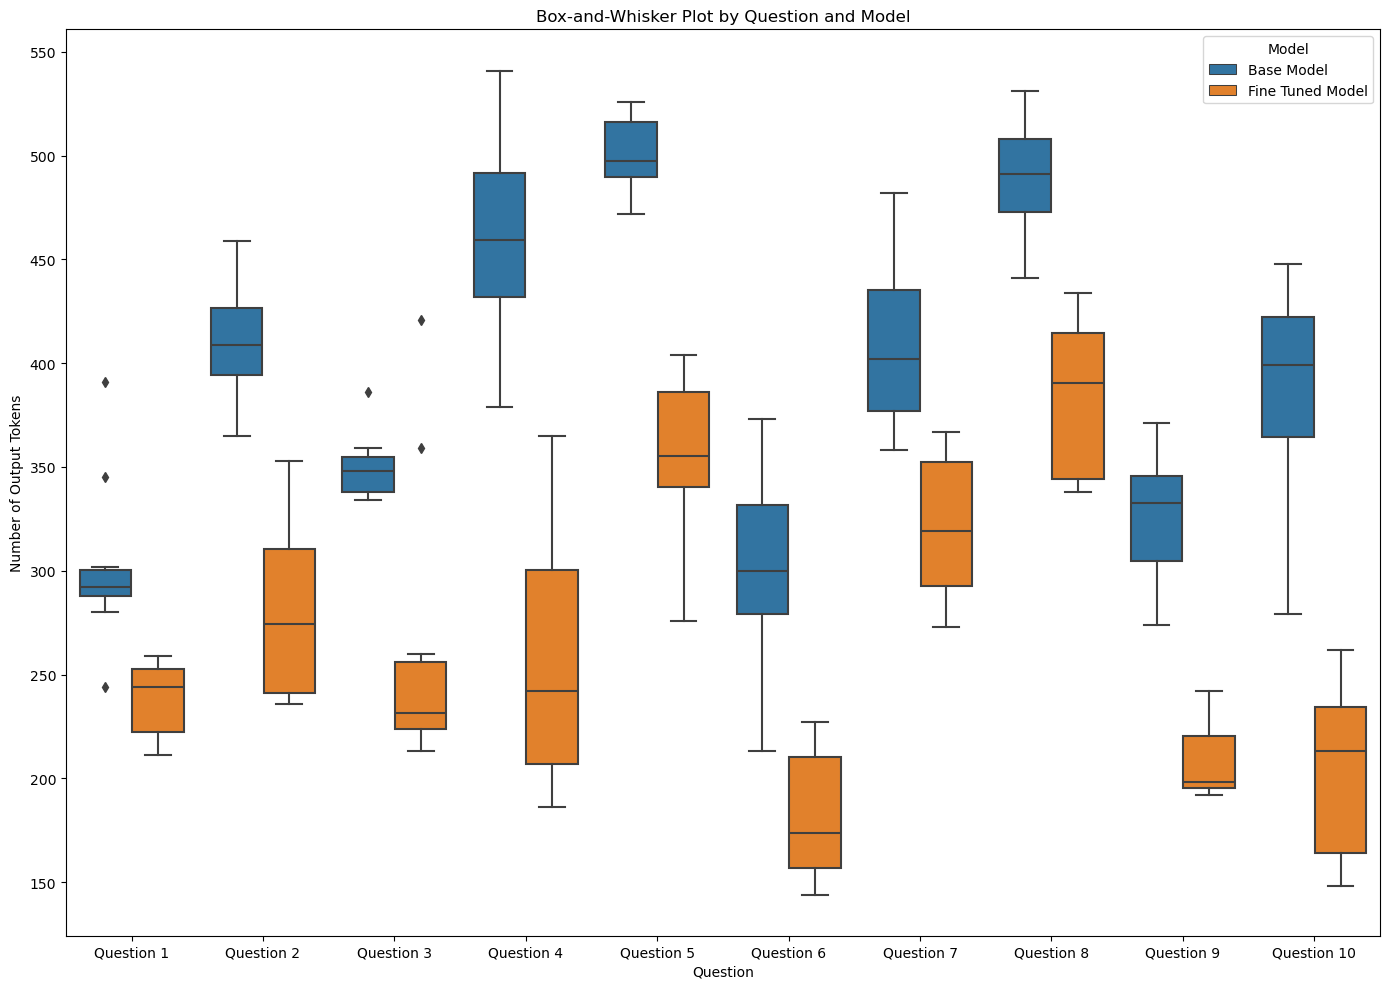
\includegraphics[width=0.9\textwidth]{Figures/Box-and-Whisker Plot by Question and Model.png}
    \caption{Average number of tokens by question: Base vs.\ Fine-Tuned Model.}
    \label{fig:avg-token-by-question}
\end{figure}


This observation is further substantiated by Figure~\ref{fig:avg-tokens-by-question}, which explicitly compares average token usage per question between the two models. he bar chart comparing token usage between the Base Model and Fine-Tuned Model indicates that the Fine-Tuned Model consistently produces shorter outputs across all ten questions (Q1–Q10), suggesting that fine-tuning led to more concise outputs. Notably, the difference in token usage is especially large in some questions (e.g., Q4, Q5, and Q10), indicating that certain question types or complexities might benefit more from the fine-tuning process. For example, in Q4 the Base Model uses 460.3 tokens while the Fine-Tuned Model uses only 257.2 tokens—a reduction of over 200 tokens. Similarly, Q5 shows a drop from 499.8 tokens in the Base Model to 355.8 in the Fine-Tuned Model, and Q10 decreases from 384.5 to 204 tokens, illustrating substantial efficiency improvements. Although some questions like Q1 and Q3 have more moderate differences—301.7 tokens versus 239 in Q1, and 350 versus 262.9 in Q3—these examples still underscore the overall trend toward reduced token consumption. This efficiency is likely attributable to focused training on domain-specific data and an enhanced capacity to avoid redundant phrasing. In practical terms, the reduction in token consumption can translate into lower inference costs and faster response times, particularly in settings where conciseness is valued. Overall, the visualization demonstrates that fine-tuning can optimize token usage, offering tangible benefits in terms of cost and computational efficiency.

\begin{figure}[H]
    \centering
    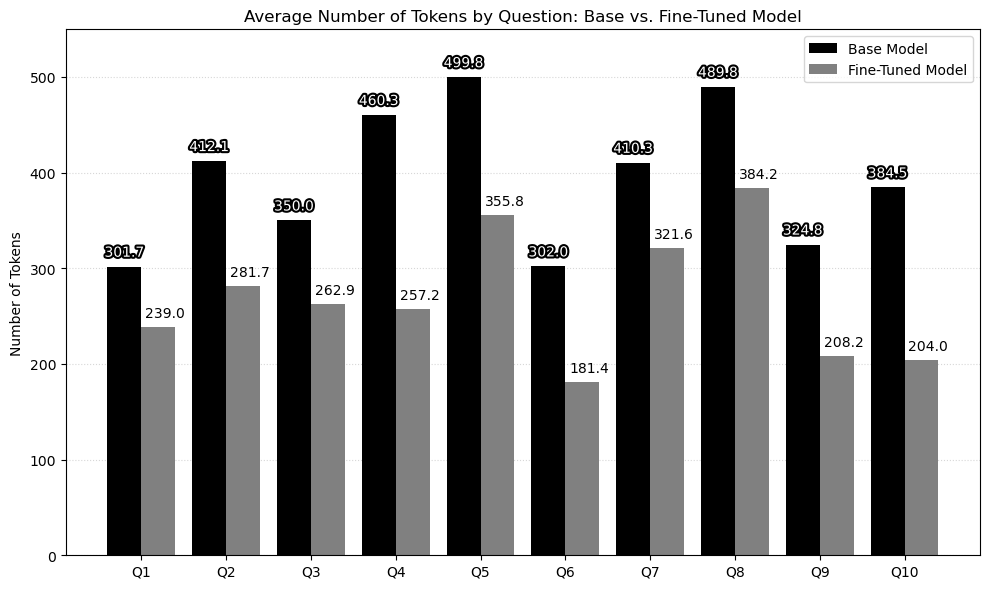
\includegraphics[width=0.8\textwidth]{Figures/Average Number of Tokens by Question.png}
    \caption{Average number of tokens by question: Base vs.\ Fine-Tuned Model.}
    \label{fig:avg-tokens-by-question}
\end{figure}


Cost efficiency, directly correlated to token usage, is depicted in Figure~\ref{fig:avg-cost-by-question}, which compares the average output cost per question. Consistently, the base model incurred higher costs than the fine-tuned model across every question. This visualization presents the token costs for generating outputs on ten identical questions, comparing the Base Model (black bars) and the Fine-Tuned Model (gray bars). The x-axis lists questions Q1 through Q10, while the y-axis quantifies the cost in U.S. dollars. For every question, the Base Model consistently incurs a higher cost than the Fine-Tuned Model. For example, in Q1, the Base Model costs 0.003017 USD compared to 0.002390 USD for the Fine-Tuned Model. This pattern holds across the board: Q4 shows a Base Model cost of 0.004603 USD versus 0.002572 USD for the Fine-Tuned Model, and Q10 reveals a cost of 0.003845 USD for the Base Model against 0.002040 USD for the Fine-Tuned Model. Even where the costs are generally lower, as seen in Q6 (0.003020 USD for the Base Model versus 0.001814 USD for the Fine-Tuned Model), the Fine-Tuned Model remains the less expensive option. Overall, the chart clearly demonstrates that fine-tuning reduces token usage cost on every question, emphasizing its cost efficiency in applications with high query volumes.

\begin{figure}[H]
    \centering
    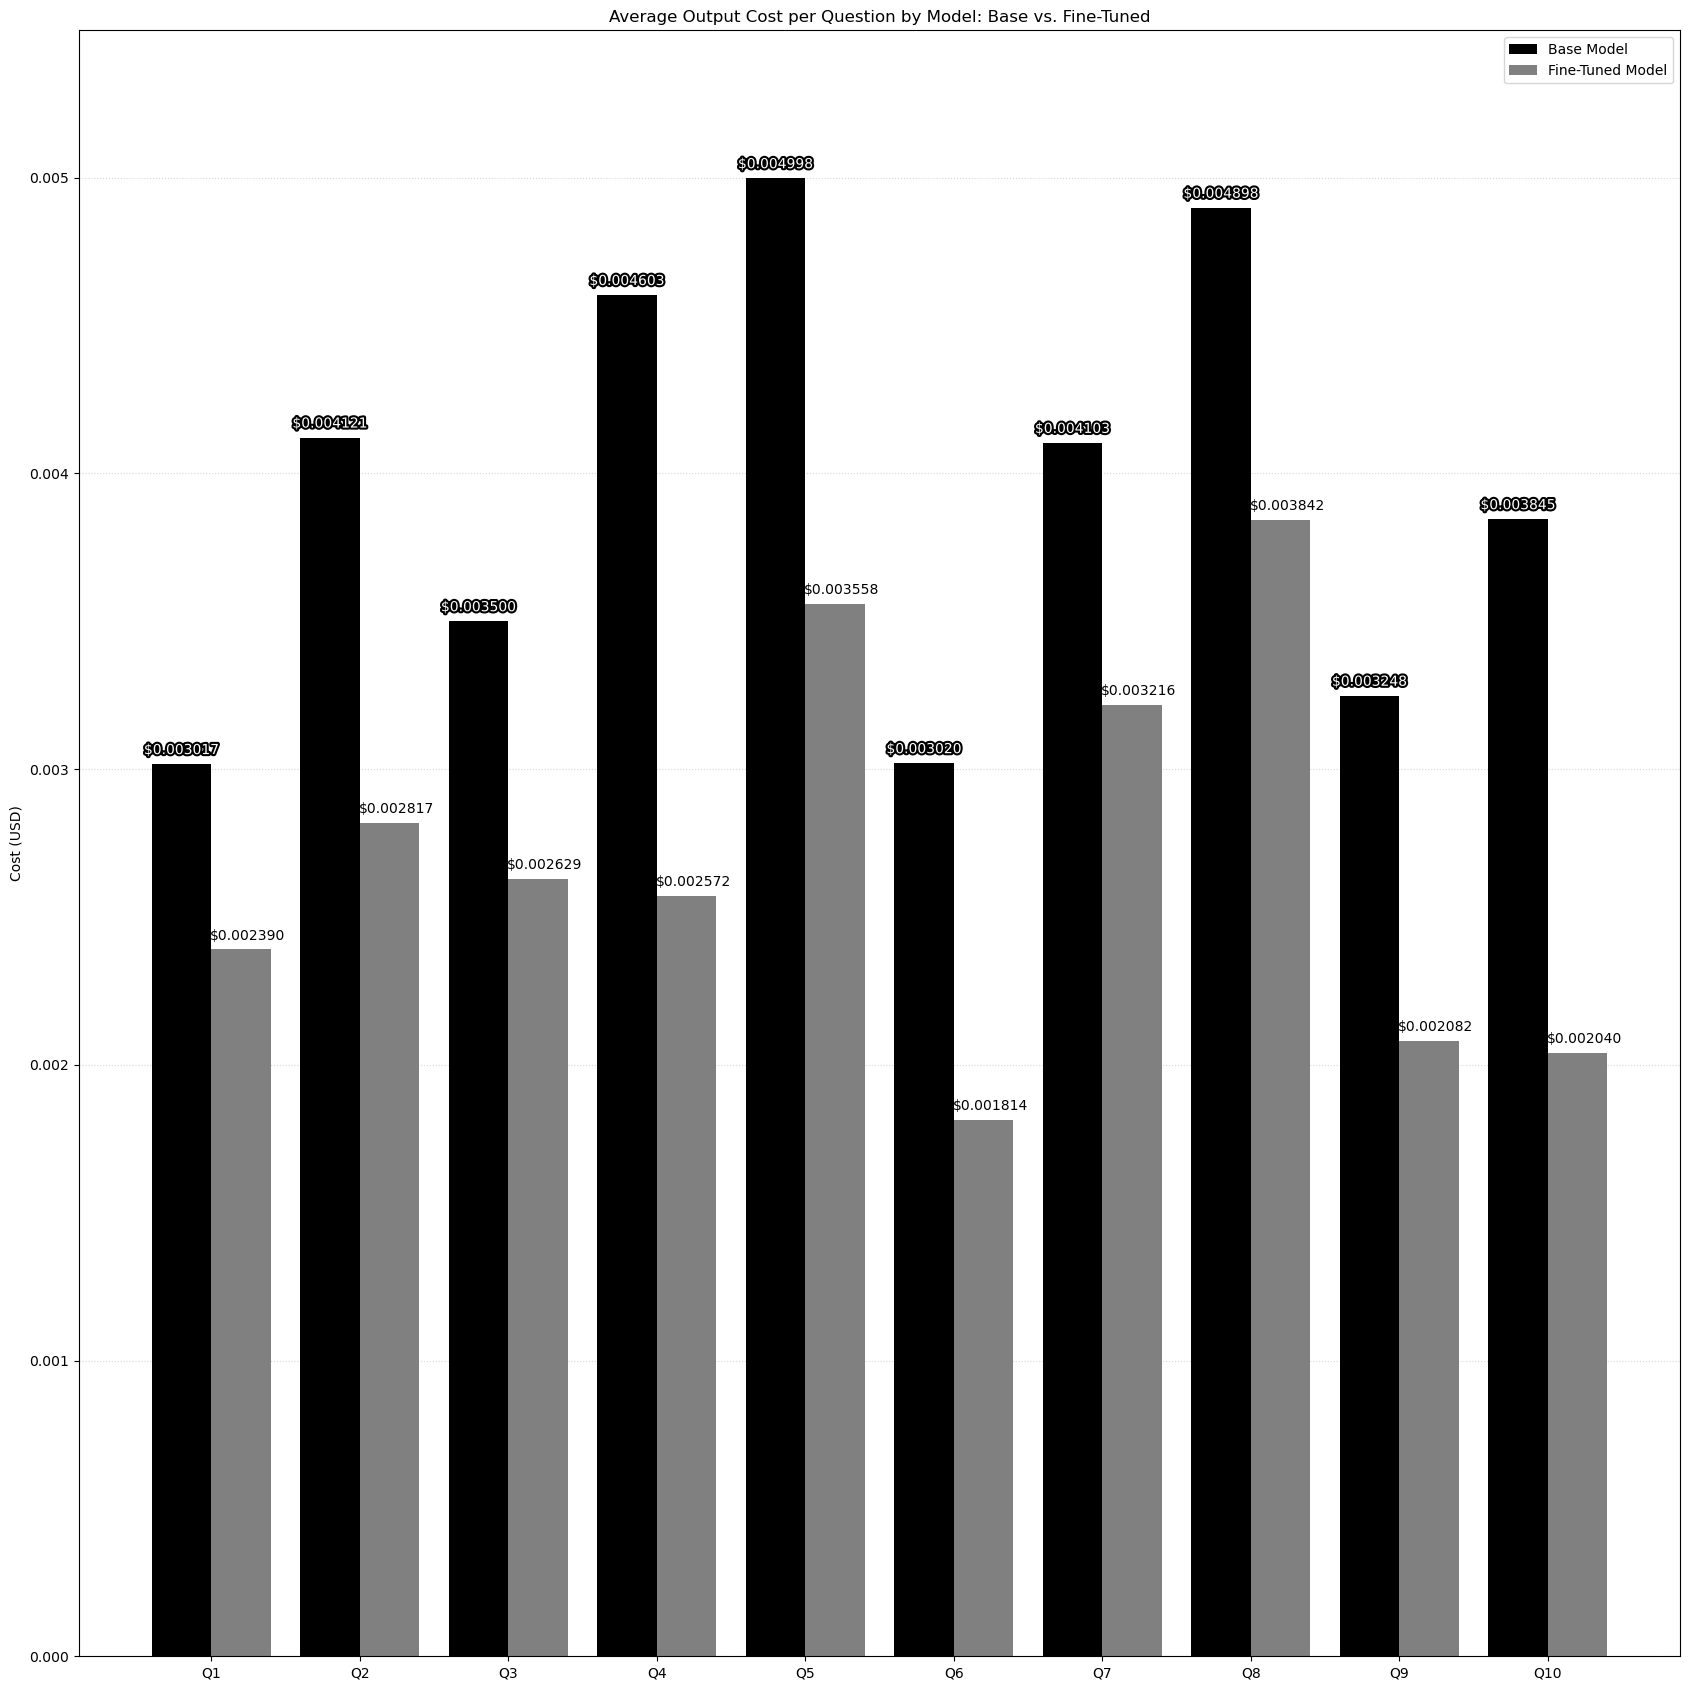
\includegraphics[width=0.7\textwidth]{Figures/Average Output Cost per Question by Model.png}
    \caption{Average cost of tokens by question: Base vs.\ Fine-Tuned Model.}
    \label{fig:avg-cost-by-question}
\end{figure}

A broader perspective on efficiency is provided by Figure~\ref{fig:total-tokens-by-model}, which compares the total output token consumption between the two models. The base model was found to generate 39,353 tokens, whereas the fine-tuned model yielded 26,960 tokens, indicating a \verb|31.5%| reduction in token usage. This decrease suggests a more efficient utilization of resources, as fewer tokens typically imply reduced computational overhead and potentially faster processing times. Such findings underscore the advantages of fine-tuning, particularly in contexts where system performance and resource constraints are of critical importance.


\begin{figure}[H]
    \centering
    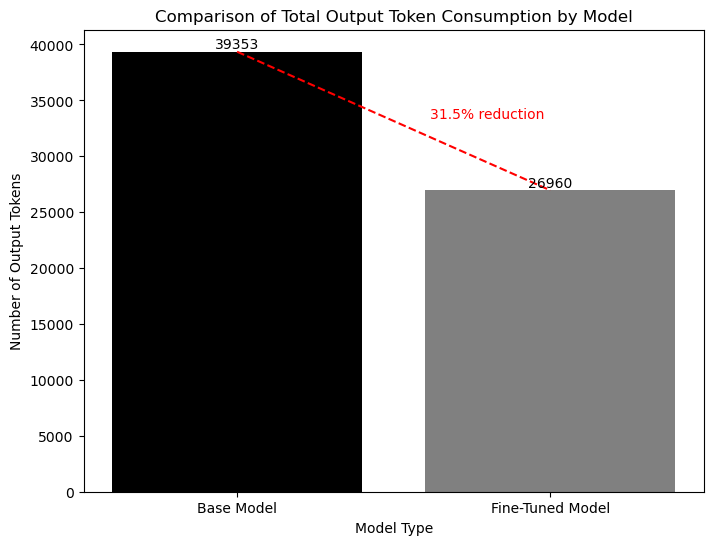
\includegraphics[width=0.9\textwidth]{Figures/Comparison of Total Output Token Consumption by Model.png}
    \caption{Total number of output tokens used by models: Base vs.\ Fine-Tuned Model.}
    \label{fig:total-tokens-by-model}
\end{figure}


Similarly, Figure~\ref{fig:avg-output-tokens}compares the average token output of the Base Model (black bar) to that of the Fine-Tuned Model (gray bar). The height of each bar reflects the mean number of tokens generated per question (using your “total tokens per question” data as the basis). From the chart:

\begin{itemize}

     \item The Base Model averages around 3935 tokens.
     
     \item The Fine-Tuned Model averages around 2696 tokens.
\end{itemize}
     
The dashed line indicates there is roughly a \verb|31.5%| reduction in token usage when moving from the Base Model to the Fine-Tuned Model. In other words, on average, the Fine-Tuned Model produces significantly fewer tokens—suggesting more concise responses and potentially lower computational costs.


\begin{figure}[H]
    \centering
    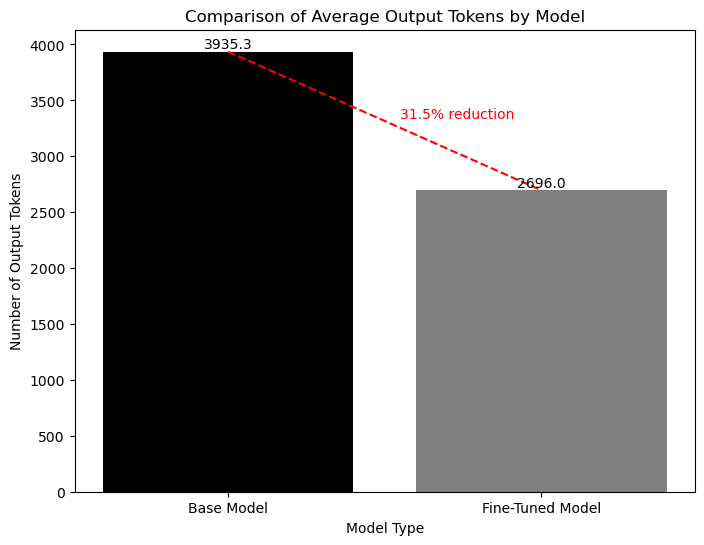
\includegraphics[width=0.7\textwidth]{Figures/Comparison of Average Output Tokens by Model.png}
    \caption{Comparison of Average Output Tokens by Model.}
    \label{fig:avg-output-tokens}
\end{figure}


\begin{figure}[ht]
    \centering
    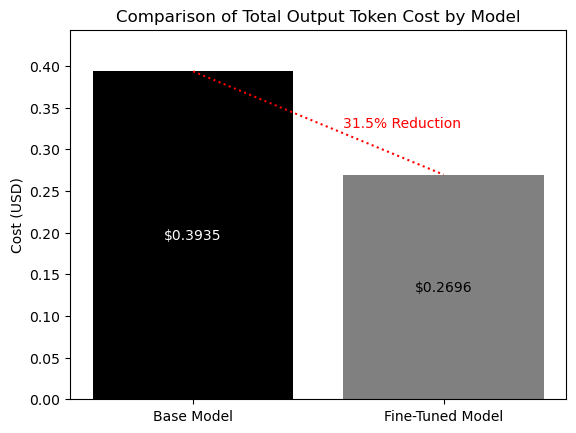
\includegraphics[width=0.7\textwidth]{Figures/Comparison of Total Output Token Cost by Model.png}
    \caption{Comparison of Total Output Token Cost by Model.}
    \label{fig:output-token-cost}
\end{figure}

Finally, the overall financial implications of these efficiency improvements are summarized in Figure \ref{fig:output-token-cost}. Each bar shows the overall expense associated with generating output tokens for the same set of questions or tasks. 

\begin{itemize}
    

    \item Base Model: costs approximately \verb|$|0.3935.
    \item Fine-Tuned Model: costs approximately \verb|$|0.2696.

\end{itemize}
The dashed line indicates about a \verb|31.5%| cost reduction when switching from the Base Model to the Fine-Tuned Model. In other words, the Fine-Tuned Model’s output tokens are more cost-effective, implying you get the same or similar results at a significantly lower cost.

\chapter{FUTURE WORK}
The system created has shown significant improvements in cost efficiency, performance, and accuracy through fine-tuning and token optimization, but there are several areas for future research and enhancement. Expanding the academic advising sytem across different academic departments and programs would help test its scalability and ability to generalize effectively. Additionally, using advanced memory systems like vector databases could improve how the chatbot remembers past conversations and maintains context. Developing an automated system for continuous learning would allow the chatbot to adapt dynamically to student feedback and changes in academic policies. Conducting detailed user studies with students, involving systematic testing scenarios and surveys, could provide deeper insights into user satisfaction, interaction patterns, and the effectiveness of recommendations. Further research into advanced token optimization methods could help reduce operational costs without affecting the quality of responses. Finally, exploring and adopting newer language models could further enhance the system's flexibility and overall effectiveness.



\addcontentsline{toc}{chapter}{BIBLIOGRAPHY}
\bibliographystyle{plain}
\bibliography{Bulut}



% Appendix
\appendix


\chapter{Appendix:Model Details}

In this appendix, visual representations of key code segments utilized in the project are presented. The first image displays the implementation of the base model, while the second image illustrates the fine-tuned model. The images offer an overview of the coding structure and the parameters applied in each model.

\begin{figure}[H]
    \centering
    \includegraphics[width=0.5\textwidth]{Figures/Base Model Code.png}
    \caption{Base Model Code}
    \label{fig:base_model_code}
\end{figure}

\begin{figure}[H]
    \centering
    \includegraphics[width=0.5\textwidth]{Figures/Fine Tuned Model Code.png}
    \caption{Fine-Tuned Model Code}
    \label{fig:fine_tuned_model_code}
\end{figure}

\chapter{Appendix: Identical Evaluation Questions for Both Models}

\begin{enumerate}[leftmargin=*, label=\textbf{\arabic*.}]
    \item \textbf{Core Curriculum and Prerequisites:} “What are the core courses required for my MScIS program, and do any of them have specific prerequisites I need to complete before enrolling?”
    \item \textbf{Credit Completion:} “How many credits do I still need to earn in order to complete my degree, and which courses are available to help me reach that total?”
    \item \textbf{Restricted Credit Hours:} “I noticed that no more than 9 credit hours from courses like CSC 591, MIS 591, CSC 595, MIS 595, CSC 598, and MIS 598 can be applied toward my degree—can you explain how that works?”
    \item \textbf{Additional Course Options:} “What are my options for fulfilling the additional course requirement, and are there any restrictions—such as specific courses that cannot be used (for example, excluding CSC 594 or MIS 594)?”
    \item \textbf{Research Project vs. Thesis:} “Can you explain the differences between the research project and thesis options for meeting the research/thesis credit requirement, and what are the key milestones for each?”
    \item \textbf{Graduation Requirements:} “Beyond completing the required credits, what additional graduation requirements should I be aware of (such as applying to graduate on SeaNet and enrolling in the semester of graduation)?”
    \item \textbf{GPA Concerns:} “Since I currently do not meet the minimum 3.0 GPA requirement for my major, what strategies or options are available to help me improve my academic standing?”
    \item \textbf{International Student Enrollment and Visa Compliance:} “As an international student, I’m concerned about maintaining my visa status while managing my academic progress. Could you explain how my course schedule and prerequisites are structured to ensure I remain a full-time student, and what additional steps or documentation might be necessary to meet both academic and immigration requirements?”
    \item \textbf{Course Repetition:} “If I do not achieve the required grade in a course, is it possible to repeat it, and how would that affect my overall credit count and GPA?”
    \item \textbf{Course Scheduling and Availability:} “Are there specific scheduling guidelines or typical semester offerings for required courses like Network Programming (CSC 544) and Database Management Systems (MIS 555) that I should plan for?”
\end{enumerate}

\chapter{Appendix:Data Storage} 


All text data files used in this analysis were systematically organized into folders based on key parameters: whether the content comprised questions (stored as \texttt{General(Base) Model Questions} or \texttt{Fine Tuned Model Questions}), the specific question number (e.g., \texttt{Question1}, \texttt{Question2}, …, \texttt{Question10}), and the  iteration number associated with each question (e.g., \texttt{Time1}, \texttt{Time2}, …, \texttt{Time5}).


\begin{figure}[htbp]
  \centering
  \includegraphics[width=0.7\textwidth]{Figures/Folders_txt.png}
  \caption{Data Stroge Folders}
  \label{fig:folders}
\end{figure}

\begin{figure}[htbp]
  \centering
  \includegraphics[width=0.7\textwidth]{Figures/Example Txt File.png}
  \caption{As here in the example figure from a fine tuned model output example for question1 and 1st run.}
  \label{fig:example}
\end{figure}

\chapter{Appendix:Token Calculation} 


\begin{figure}[htbp]
    \centering
    \includegraphics[width=0.8\textwidth]{Figures/Token Claculation Code.png}
    \caption{Part of the code and example output for token calculation.}
    \label{fig:token-calculation}
\end{figure}



\end{document}
